\documentclass[10.5pt,a4paper]{article}

\usepackage{mathptmx}
\usepackage{amsmath,amssymb}
\usepackage{graphicx}
\usepackage{booktabs}
\usepackage[margin=2.2cm]{geometry}
\usepackage[font=small,labelfont=bf]{caption}
\usepackage[colorlinks=true,linkcolor=blue,citecolor=blue,urlcolor=blue]{hyperref}

\graphicspath{{../figures/}}

% ---------- Macros ----------
\newcommand{\ket}[1]{\left|#1\right\rangle}
\newcommand{\bra}[1]{\left\langle #1\right|}
\newcommand{\Tr}{\operatorname{Tr}}
\newcommand{\Var}{\operatorname{Var}}
\newcommand{\FQ}{F_Q}
\newcommand{\Neg}{\mathcal N}

% 2x2 figure: \figfour{a}{b}{c}{d}{caption}
\newcommand{\figfour}[6]{%
  \begin{figure}[t]
    \centering
    \includegraphics[width=0.49\textwidth]{#1}\hfill
    \includegraphics[width=0.49\textwidth]{#2}\\[2pt]
    \includegraphics[width=0.49\textwidth]{#3}\hfill
    \includegraphics[width=0.49\textwidth]{#4}
    \caption{#5}\label{#6}
  \end{figure}}

\title{Entanglement Dynamics and Quantum Metrology\\in a Two-Qubit Heisenberg XXZ Model}
\author{Dhimen Nabil\\[2pt]
\small Master in Mathematical Physics, Faculty of Sciences, Mohammed V University, Rabat, Morocco\\
\small LPHE -- Mod\'elisation et Simulation}
\date{}

\begin{document}
\maketitle

\begin{abstract}
\noindent We study entanglement dynamics and quantum metrology in a two-qubit Heisenberg XXZ model for four initial pure states chosen to cover the symmetry sectors of the Hamiltonian: a stationary product state, a product state that becomes maximally entangled, a product state that reaches only partial entanglement, and a stationary maximally entangled state. Concurrence, negativity and the purity of the reduced states are obtained in closed form. When the parameter to be estimated is encoded by the total $S_z$, which commutes with the Hamiltonian, the quantum Fisher information (QFI) is $\FQ=4t^2\Var(S_z)$, the anisotropy $\Delta$ enters only through phases, and entanglement plays no role. When it is encoded by the total $S_x$, which does not commute with the Hamiltonian, $\Delta$ enters through the detuning $\omega=2J(1-\Delta)$ and the Bell state gives exactly twice the QFI of the product states. Adding local dephasing described by a Lindblad equation, we find no sudden death of entanglement. The Bell-state advantage shrinks, from $2.00$ to $1.51$ at the best interrogation time for a dephasing rate $\gamma=0.5$, but it survives there; at long times the product states $\ket{00}$, $\ket{01}$ and the Bell state reach the same QFI. All results are checked with independent numerical methods.
\end{abstract}

% ====================================================================
\section{Introduction}
% ====================================================================

Heisenberg-type spin models are the simplest interacting quantum systems in which entanglement is generated dynamically, and they are a standard testbed for quantum information protocols \cite{Horodecki2009}. In the two-qubit case the dynamics can be solved in closed form, so that analytic results can be compared with numerical simulations and one can see exactly which feature of the model controls each quantity.

Entanglement is often presented as a resource for quantum metrology, that is, for estimating a parameter with a precision beyond what is possible with product states \cite{Giovannetti2011}. Whether a given amount of entanglement actually translates into a larger quantum Fisher information (QFI) depends on how the parameter is encoded and on the noise. In this work we examine this question in the simplest dynamical setting: two qubits coupled by an XXZ interaction, four initial states that span the structure of the dynamics, a parameter encoded either by a conserved or by a non-conserved generator, and local dephasing.

The paper is organised as follows. Section~\ref{sec:model} introduces the model, its symmetry sectors and the four initial states. Section~\ref{sec:ent} gives the entanglement and purity dynamics. Section~\ref{sec:comm} treats the metrological problem for a generator that commutes with the Hamiltonian. Section~\ref{sec:noncomm} replaces it by one that does not commute and adds local dephasing. Section~\ref{sec:disc} summarises the results and their limitations. The calculations are standard; the contribution of this work is a complete, quantitative and numerically cross-checked characterisation of these four states. The full hand derivations, including the explicit density matrices of every state, are given in the accompanying technical report.

% ====================================================================
\section{Model and initial states}\label{sec:model}
% ====================================================================

We use $\hslash=1$ and
\begin{equation}
  H=J\left(\sigma_x\otimes\sigma_x+\sigma_y\otimes\sigma_y+\Delta\,\sigma_z\otimes\sigma_z\right),
  \label{eq:H}
\end{equation}
where $\sigma_{x,y,z}$ are Pauli matrices, $J$ is the coupling and $\Delta$ the anisotropy. Numerically $J=1$ and $\Delta=0.5$. In the ordered basis $\{\ket{00},\ket{01},\ket{10},\ket{11}\}$,
\begin{equation}
  H=J\begin{pmatrix}\Delta&0&0&0\\0&-\Delta&2&0\\0&2&-\Delta&0\\0&0&0&\Delta\end{pmatrix}.
\end{equation}
Its eigenvectors and eigenvalues are $\ket{00}$ and $\ket{11}$ with $E=J\Delta$, and $\ket{\psi_\pm}=(\ket{01}\pm\ket{10})/\sqrt2$ with $E_\pm=-J\Delta\pm2J$. Since Pauli matrices are used instead of spin-$1/2$ operators, the characteristic frequency is $4J$.

\paragraph{Symmetry sectors.}
The total spin component $S_z=\tfrac12(\sigma_z\otimes I+I\otimes\sigma_z)$ commutes with $H$, so its eigenvalue $M$ is conserved and the Hilbert space splits into $M=+1:\{\ket{00}\}$, $M=0:\{\ket{01},\ket{10}\}$ and $M=-1:\{\ket{11}\}$. In each sector $\sigma_z\otimes\sigma_z$ is constant ($+1,-1,+1$), so the $\Delta$ term gives a constant energy per sector. The anisotropy is therefore a \emph{global} phase for a state in a single sector and a \emph{relative} phase between sectors otherwise. The exchange term acts only in the $M=0$ sector, which is where entanglement is generated.

\paragraph{Initial states.}
We study
\begin{equation}
  \ket{00},\qquad \ket{01},\qquad \tfrac{1}{\sqrt2}\bigl(\ket{00}+\ket{01}\bigr),\qquad \ket{\psi_+}.
\end{equation}
They were chosen to cover the structure of the dynamics: a stationary product state (control), a product state that evolves into a maximally entangled state, a product state that reaches partial entanglement through a superposition of two sectors, and a stationary maximally entangled state (control).

% ====================================================================
\section{Entanglement and purity dynamics}\label{sec:ent}
% ====================================================================

For a pure state $\ket\psi=\sum_{ij}c_{ij}\ket{ij}$ the concurrence is $C=2\lvert c_{00}c_{11}-c_{01}c_{10}\rvert$, which vanishes if and only if the state is separable; for mixed states we use Wootters' formula \cite{Wootters1998}. The negativity is $\Neg(\rho)=\sum_{\mu_i<0}\lvert\mu_i\rvert$, the sum of the absolute values of the negative eigenvalues of the partial transpose $\rho^{T_B}$ \cite{VidalWerner2002}. For every pure two-qubit state, with Schmidt coefficients $\lambda_{1,2}$, the spectrum of $\rho^{T_B}$ is $\{\lambda_1,\lambda_2,\pm\sqrt{\lambda_1\lambda_2}\}$, so $\Neg=\sqrt{\lambda_1\lambda_2}$ and $C=2\sqrt{\lambda_1\lambda_2}$, that is
\begin{equation}
  \Neg=\frac C2,\qquad P_A=P_B=\lambda_1^2+\lambda_2^2=1-\frac{C^2}{2},
  \label{eq:NCP}
\end{equation}
where $P_{A}=\Tr\rho_A^2$ is the purity of the reduced state of qubit $A$.

\paragraph{Time evolution.}
Write $c=\cos 2Jt$ and $s=\sin 2Jt$. The state $\ket{00}$ is an eigenvector and only acquires a global phase. Inside the $M=0$ sector $H=-J\Delta\,I+2J\,\sigma_x'$, where $\sigma_x'$ exchanges $\ket{01}$ and $\ket{10}$, so
\begin{align}
  \ket{01}&\to e^{iJ\Delta t}\bigl[c\ket{01}-is\ket{10}\bigr],\\
  \tfrac{1}{\sqrt2}\bigl(\ket{00}+\ket{01}\bigr)&\to\tfrac{1}{\sqrt2}\Bigl[e^{-iJ\Delta t}\ket{00}+e^{iJ\Delta t}\bigl(c\ket{01}-is\ket{10}\bigr)\Bigr],
\end{align}
and $\ket{\psi_+}$ is an eigenvector with energy $2J-J\Delta$. For the first state, $\rho(t)$ contains the coherence $ics$ between $\ket{01}$ and $\ket{10}$; the partial transpose moves it to the corners of the matrix, giving the spectrum $\{c^2,s^2,cs,-cs\}$ and $\Neg=\lvert cs\rvert=\tfrac12\lvert\sin4Jt\rvert$. For the superposition state the phase $e^{-2iJ\Delta t}$ between the two sectors appears in $\rho$ but not in its spectrum. Since $c_{11}=0$ in all cases, $C=2\lvert c_{01}c_{10}\rvert$ gives the results of Table~\ref{tab:ent}, and Eq.~\eqref{eq:NCP} is verified in each case.

\begin{table}[t]
  \centering
  \begin{tabular}{@{}lccccc@{}}
    \toprule
    Initial state & $C(t)$ & $\Neg(t)$ & $P_A(t)=P_B(t)$ & $P_{\min}$ & Role of $\Delta$\\
    \midrule
    $\ket{00}$ & $0$ & $0$ & $1$ & $1$ & global phase\\
    $\ket{01}$ & $\lvert\sin4Jt\rvert$ & $\tfrac12\lvert\sin4Jt\rvert$ & $1-\tfrac12\sin^24Jt$ & $1/2$ & global phase\\
    $(\ket{00}+\ket{01})/\sqrt2$ & $\tfrac12\lvert\sin4Jt\rvert$ & $\tfrac14\lvert\sin4Jt\rvert$ & $1-\tfrac18\sin^24Jt$ & $7/8$ & relative phase\\
    $\ket{\psi_+}$ & $1$ & $1/2$ & $1/2$ & $1/2$ & global phase\\
    \bottomrule
  \end{tabular}
  \caption{Closed-form entanglement and purity dynamics of the four initial states. $\Delta$ never changes $C$, $\Neg$ or $P$ for these states.}
  \label{tab:ent}
\end{table}

\figfour{state1_entanglement.pdf}{state2_entanglement.pdf}{state3_entanglement.pdf}{state4_entanglement.pdf}{Concurrence and negativity for the four initial states ($J=1$, $\Delta=0.5$): $\ket{00}$, $\ket{01}$ (top), $(\ket{00}+\ket{01})/\sqrt2$, $\ket{\psi_+}$ (bottom).}{fig:ent}

For $\ket{01}$ the pair is maximally entangled whenever $\lvert\sin4Jt\rvert=1$ and returns to a product state at $4Jt=k\pi$; each qubit is then maximally mixed ($\rho_A=\rho_B=\tfrac12I$). For $(\ket{00}+\ket{01})/\sqrt2$ only half of the weight lies in the $M=0$ sector, which caps the concurrence at $C_{\max}=1/2$. The state $\ket{\psi_+}$ is protected by the dynamics, $C=1$ at all times and $\rho_A=\rho_B=\tfrac12 I$. Three points emerge. Entanglement generation requires a component in the $M=0$ sector, and its maximum is set by the weight of the state in that sector. The initial state, not $\Delta$, controls the amplitude of entanglement. The reduced purity decreases exactly when entanglement increases, as Eq.~\eqref{eq:NCP} states.

% ====================================================================
\section{Quantum Fisher information for a commuting generator}\label{sec:comm}
% ====================================================================

Let a pure state $\ket{\psi_\lambda}$ depend on a parameter $\lambda$. Its QFI is $\FQ=4\bigl(\langle\partial_\lambda\psi_\lambda|\partial_\lambda\psi_\lambda\rangle-\lvert\langle\psi_\lambda|\partial_\lambda\psi_\lambda\rangle\rvert^2\bigr)$, and for $\nu$ independent repetitions any unbiased estimator obeys the quantum Cram\'er--Rao bound \cite{BraunsteinCaves1994,Giovannetti2011}
\begin{equation}
  \delta\lambda\ \ge\ \delta\lambda_{\min}=\frac{1}{\sqrt{\nu\,\FQ}}.
\end{equation}
The bound depends only on the state family; saturating it requires an optimal measurement. We use $\nu=1000$.

We encode $\lambda$ by $H(\lambda)=H_{XXZ}+\lambda V$ with $V=S_z$. Since $[H_{XXZ},V]=0$, the evolution factorises, $e^{-iH(\lambda)t}=e^{-iH_{XXZ}t}e^{-i\lambda Vt}$, so $\partial_\lambda\ket{\psi_\lambda}=-itV\ket{\psi_\lambda}$ and
\begin{equation}
  \FQ(t)=4t^2\,\Var(V).
  \label{eq:FQ}
\end{equation}
The variance is conserved and can be computed in the initial state. It vanishes for every state in a single $M$ sector. Hence $\FQ=0$ for $\ket{00}$, $\ket{01}$ and $\ket{\psi_+}$, so that no finite bound exists, while the equal superposition of $M=+1$ and $M=0$ has $\langle V\rangle=\langle V^2\rangle=1/2$, $\Var(V)=1/4$, and
\begin{equation}
  \FQ(t)=t^2,\qquad \delta\lambda_{\min}(t)=\frac{1}{t\sqrt\nu}.
\end{equation}
Neither $J$ nor $\Delta$ appears: the interaction does not encode $\lambda$. A vanishing $\FQ$ means that the state is insensitive to $\lambda$ through this particular encoding, not that it carries no quantum information. Remarkably, the only state with $\FQ\neq0$ is a product state, while the maximally entangled state $\ket{\psi_+}$ gives $\FQ=0$: for this generator, entanglement and metrological usefulness are unrelated, as a consequence of the conservation of $S_z$.

% ====================================================================
\section{Non-commuting encoding and local dephasing}\label{sec:noncomm}
% ====================================================================

We now lift both simplifications: the parameter is encoded by $V=S_x=\tfrac12(\sigma_x\otimes I+I\otimes\sigma_x)$, and each qubit is subject to local dephasing. The same four initial states are used, with $J=1$, $\Delta=0.5$, $\nu=1000$ and $t\in[0,4\pi]$.

\subsection{Non-commuting generator without noise}
A direct computation gives
\begin{equation}
  [H_{XXZ},S_x]=iJ(\Delta-1)\bigl(\sigma_z\otimes\sigma_y+\sigma_y\otimes\sigma_z\bigr),
\end{equation}
which is non-zero for $\Delta\neq1$; at $\Delta=1$ the Hamiltonian is the isotropic Heisenberg model and $[H,S_x]=0$ again. Because the exponent no longer factorises, we use the Duhamel formula: $\partial_\lambda\ket{\psi_\lambda(t)}\big|_{\lambda=0}=-i\,e^{-iHt}G(t)\ket{\psi(0)}$ with $G(t)=\int_0^te^{iHs}Ve^{-iHs}ds$, so that
\begin{equation}
  \FQ(t)=4\Var_{\psi(0)}\bigl(G(t)\bigr).
\end{equation}
In the eigenbasis of $H$, $G_{mn}=V_{mn}(e^{i\omega_{mn}t}-1)/(i\omega_{mn})$ for $\omega_{mn}=E_m-E_n\neq0$. The states $\ket{00}$ and $\ket{\psi_+}$ are eigenstates with $\langle S_x\rangle=0$, and $S_x\ket{00}=\ket{\psi_+}/\sqrt2$, $S_x\ket{\psi_+}=(\ket{00}+\ket{11})/\sqrt2$. With $\omega=E_{\psi_+}-E_{00}=2J(1-\Delta)$ we obtain
\begin{equation}
  \FQ^{(00)}(t)=\frac{8\sin^2(\omega t/2)}{\omega^2},\qquad
  \FQ^{(\psi_+)}(t)=\frac{16\sin^2(\omega t/2)}{\omega^2}=2\,\FQ^{(00)}(t).
  \label{eq:FQclosed}
\end{equation}
For $\Delta=0.5$, $\omega=1$. Three consequences follow. First, $\Delta$ now matters: it sets the detuning between the sectors connected by $S_x$, hence the period $2\pi/\omega$ and the amplitude $\propto1/\omega^2$ of $\FQ$. Second, for $\Delta\neq1$ the QFI oscillates instead of growing as $t^2$; in the limit $\Delta\to1$ Eq.~\eqref{eq:FQclosed} gives $2t^2$ and $4t^2$, that is $Nt^2$ and $N^2t^2$ for $N=2$ qubits, the shot-noise and Heisenberg scalings. Third, the Bell state gives exactly twice the QFI of $\ket{00}$ at every time, which lowers the Cram\'er--Rao bound by $\sqrt2$. The state $\ket{01}$ gives numerically the same $\FQ(t)$ as $\ket{00}$ (the Duhamel curves agree to $3\times10^{-15}$), and for $(\ket{00}+\ket{01})/\sqrt2$ the QFI, evaluated numerically, equals $8$ at $t=\pi$ but is lower than that of $\ket{00}$ and $\ket{01}$ at the other times.

\subsection{Local dephasing}
Each qubit undergoes pure dephasing in the $z$ basis, with independent environments and rate $\gamma$:
\begin{equation}
  \dot\rho=-i\bigl[H(\lambda),\rho\bigr]+\frac\gamma2\sum_{k=A,B}\Bigl(\sigma_z^{(k)}\rho\,\sigma_z^{(k)}-\rho\Bigr),
  \label{eq:lindblad}
\end{equation}
which is of Lindblad form \cite{Lindblad1976,GKS1976,BreuerPetruccione2002}. The dephasing basis defines the conserved $S_z$, so at $\lambda=0$ the sectors $M=+1,0,-1$ remain decoupled. For mixed states the QFI is $\FQ=2\sum_{p_i+p_j>0}\lvert\langle i|\partial_\lambda\rho|j\rangle\rvert^2/(p_i+p_j)$, with $\rho=\sum_ip_i\ket i\!\bra i$ and $\partial_\lambda\rho$ at $\lambda=0$ obtained by a central finite difference; the numerical methods and checks are described in Appendix~\ref{app:num}.

\paragraph{Entanglement and sudden death.}
In the sector $\{\ket{01},\ket{10}\}$ the Bloch vector obeys, up to orientation, $\dot x=-2\gamma x$, $\dot y=-4Jz-2\gamma y$, $\dot z=4Jy$: a damped Rabi oscillation. For $\ket{01}$ and $\ket{\psi_+}$ the state stays in this sector and $C=\sqrt{x^2+y^2}$. The $M=0$ block of $(\ket{00}+\ket{01})/\sqrt2$ is half that of $\ket{01}$, so its concurrence is half as large (checked against Wootters' formula). For $\gamma<4J$ and $\Omega=\sqrt{16J^2-\gamma^2}$,
\begin{equation}
  C^{(00)}=0,\quad
  C^{(01)}=\frac{4J}{\Omega}e^{-\gamma t}\lvert\sin\Omega t\rvert,\quad
  C^{(3)}=\frac{2J}{\Omega}e^{-\gamma t}\lvert\sin\Omega t\rvert,\quad
  C^{(\psi_+)}=e^{-2\gamma t},
\end{equation}
where (3) denotes $(\ket{00}+\ket{01})/\sqrt2$. These agree with Wootters' concurrence of the numerically evolved state to $10^{-9}$ (the solver tolerance) for $\gamma\in\{0.05,0.1,0.2,0.5\}$. No finite-time disentanglement (entanglement sudden death \cite{YuEberly2004}) occurs: $\ket{\psi_+}$ loses its concurrence only asymptotically, and for $\ket{01}$ and the superposition state $C$ vanishes only at the isolated nodes $\Omega t=k\pi$, as without noise, under a smoothly decaying envelope $e^{-\gamma t}$ (Fig.~\ref{fig:conc}).

\begin{figure}[t]
  \centering
  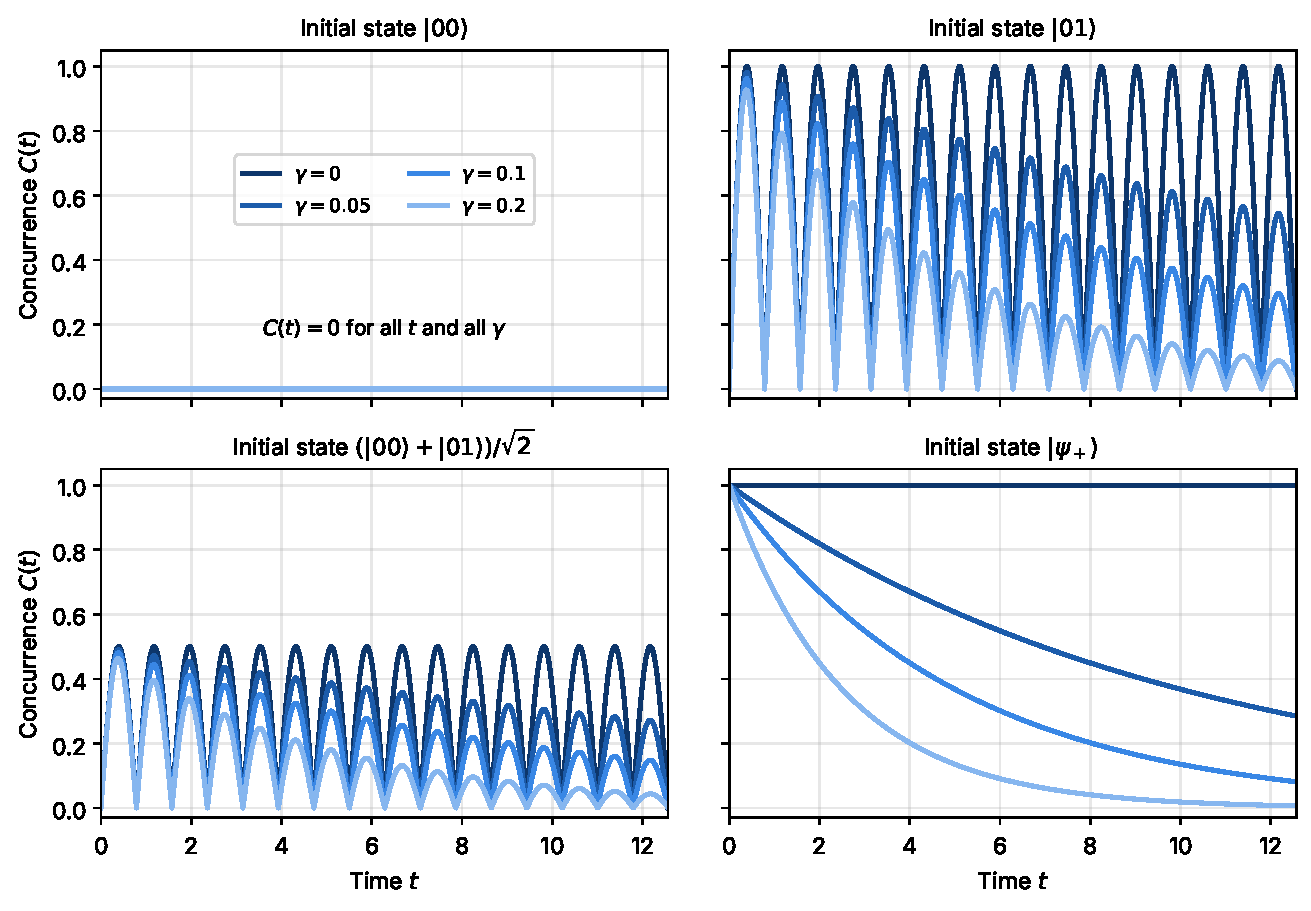
\includegraphics[width=0.62\textwidth]{nc_concurrence.pdf}
  \caption{Concurrence of the four initial states under local dephasing at $\lambda=0$, for $\gamma=0,\,0.05,\,0.1,\,0.2$ (dark to light).}
  \label{fig:conc}
\end{figure}

\subsection{QFI under dephasing}
Figure~\ref{fig:qfi} and Table~\ref{tab:peak} show the QFI for $V=S_x$. Dephasing lowers the peaks of all states. For $\ket{00}$ the first maximum moves slightly to earlier times, from $t\simeq3.14$ at $\gamma=0$ to $t\simeq2.97$ at $\gamma=0.1$. Without noise $\ket{01}$ is identical to $\ket{00}$, but with dephasing it is a few percent higher (6.24 against 5.97 at $\gamma=0.1$), so it is the more robust of the two product states. The superposition state is the most fragile (5.74 at $\gamma=0.1$ and 1.85 at $\gamma=0.5$): the coherence between the sectors $M=+1$ and $M=0$ is not protected against $z$-dephasing.

\figfour{nc_state1_QFI.pdf}{nc_state2_QFI.pdf}{nc_state3_QFI.pdf}{nc_state4_QFI.pdf}{QFI for $V=S_x$ and several dephasing rates $\gamma$, for $\ket{00}$, $\ket{01}$ (top), $(\ket{00}+\ket{01})/\sqrt2$ and $\ket{\psi_+}$ (bottom).}{fig:qfi}

\begin{table}[t]
  \centering
  \begin{tabular}{@{}lccccc@{}}
\toprule
Initial state & $\gamma=0$ & $\gamma=0.05$ & $\gamma=0.1$ & $\gamma=0.2$ & $\gamma=0.5$\\
\midrule
$\ket{00}$ & 8.00 & 6.88 & 5.97 & 4.62 & 2.47\\
$\ket{01}$ & 8.00 & 7.06 & 6.24 & 4.91 & 2.62\\
$(\ket{00}+\ket{01})/\sqrt2$ & 8.00 & 6.76 & 5.74 & 4.20 & 1.85\\
$\ket{\psi_+}$ & 16.00 & 13.65 & 11.61 & 8.46 & 3.72\\
\bottomrule
\end{tabular}

  \caption{Maximum over $t\in[0,4\pi]$ of the QFI for $V=S_x$ ($J=1$, $\Delta=0.5$).}
  \label{tab:peak}
\end{table}

\paragraph{Long times.}
For $t\gg1/\gamma$ the oscillations are damped and the QFI approaches a plateau that is the same for $\ket{00}$, $\ket{01}$ and $\ket{\psi_+}$ (Table~\ref{tab:plateau}), and well described by
\begin{equation}
  \FQ(t\to\infty)=\frac{2}{\omega^2+\gamma^2}.
\end{equation}
We found this expression empirically and have not derived it; it agrees with the numerics to four digits for $\Delta=0,\,0.25,\,0.5,\,0.75$ and $\gamma=0.1,\,0.5$. The initial state is forgotten, so any advantage of the entangled state is a finite-time effect.

\begin{table}[t]
  \centering
  \begin{tabular}{@{}lccccc@{}}
\toprule
$\gamma$ & $\ket{00}$ & $\ket{01}$ & $(\ket{00}+\ket{01})/\sqrt2$ & $\ket{\psi_+}$ & $2/(\omega^2+\gamma^2)$\\
\midrule
0.05 & 1.995 & 1.995 & 1.660 & 1.995 & 1.995\\
0.1 & 1.980 & 1.980 & 1.640 & 1.980 & 1.980\\
0.2 & 1.923 & 1.923 & 1.566 & 1.923 & 1.923\\
0.5 & 1.600 & 1.600 & 1.173 & 1.600 & 1.600\\
\bottomrule
\end{tabular}

  \caption{QFI at $t=300$ ($\Delta=0.5$). The last column is the empirical expression $2/(\omega^2+\gamma^2)$.}
  \label{tab:plateau}
\end{table}

\subsection{Cram\'er--Rao bound and entanglement advantage}
The bound $\delta\lambda_{\min}=1/\sqrt{\nu\FQ}$ diverges at the nodes of $\FQ$, so the interrogation time must be chosen near a maximum. Table~\ref{tab:crb} gives its best value over $t\in[0,4\pi]$. Without noise it is $0.0112$ for $\ket{00}$ and $0.0079$ for $\ket{\psi_+}$, a gain of $\sqrt2$; at $\gamma=0.1$ the values become $0.0129$ and $0.0093$, a gain of $1.39$. The bound is attainable only with an optimal measurement, which we do not discuss.

\begin{table}[t]
  \centering
  \begin{tabular}{@{}lccccc@{}}
\toprule
Initial state & $\gamma=0$ & $\gamma=0.05$ & $\gamma=0.1$ & $\gamma=0.2$ & $\gamma=0.5$\\
\midrule
$\ket{00}$ & 0.0112 & 0.0121 & 0.0129 & 0.0147 & 0.0201\\
$\ket{01}$ & 0.0112 & 0.0119 & 0.0127 & 0.0143 & 0.0196\\
$(\ket{00}+\ket{01})/\sqrt2$ & 0.0112 & 0.0122 & 0.0132 & 0.0154 & 0.0232\\
$\ket{\psi_+}$ & 0.0079 & 0.0086 & 0.0093 & 0.0109 & 0.0164\\
\bottomrule
\end{tabular}

  \caption{Smallest $\delta\lambda_{\min}$ over $t\in[0,4\pi]$ for $\nu=1000$.}
  \label{tab:crb}
\end{table}

Figure~\ref{fig:comp} and Table~\ref{tab:adv} compare $\ket{\psi_+}$ with $\ket{00}$. The ratio of the maximal QFI decreases from $2.00$ to $1.94$, $1.83$ and $1.51$ for $\gamma=0.1$, $0.2$ and $0.5$. If the figure of merit is the information per unit time, $\max_t\FQ/t$, the advantage is more robust: $1.98$, $1.93$ and $1.80$. The product state $\ket{00}$ has a larger QFI than $\ket{\psi_+}$ during windows around the nodes of $\FQ$, where both are small; their total duration grows with $\gamma$ (the Bell state is ahead during $82\%$ of the interval at $\gamma=0.1$ and $57\%$ at $\gamma=0.5$). At the first maximum of the QFI the Bell state remains ahead for every $\gamma$ studied.

\begin{figure}[t]
  \centering
  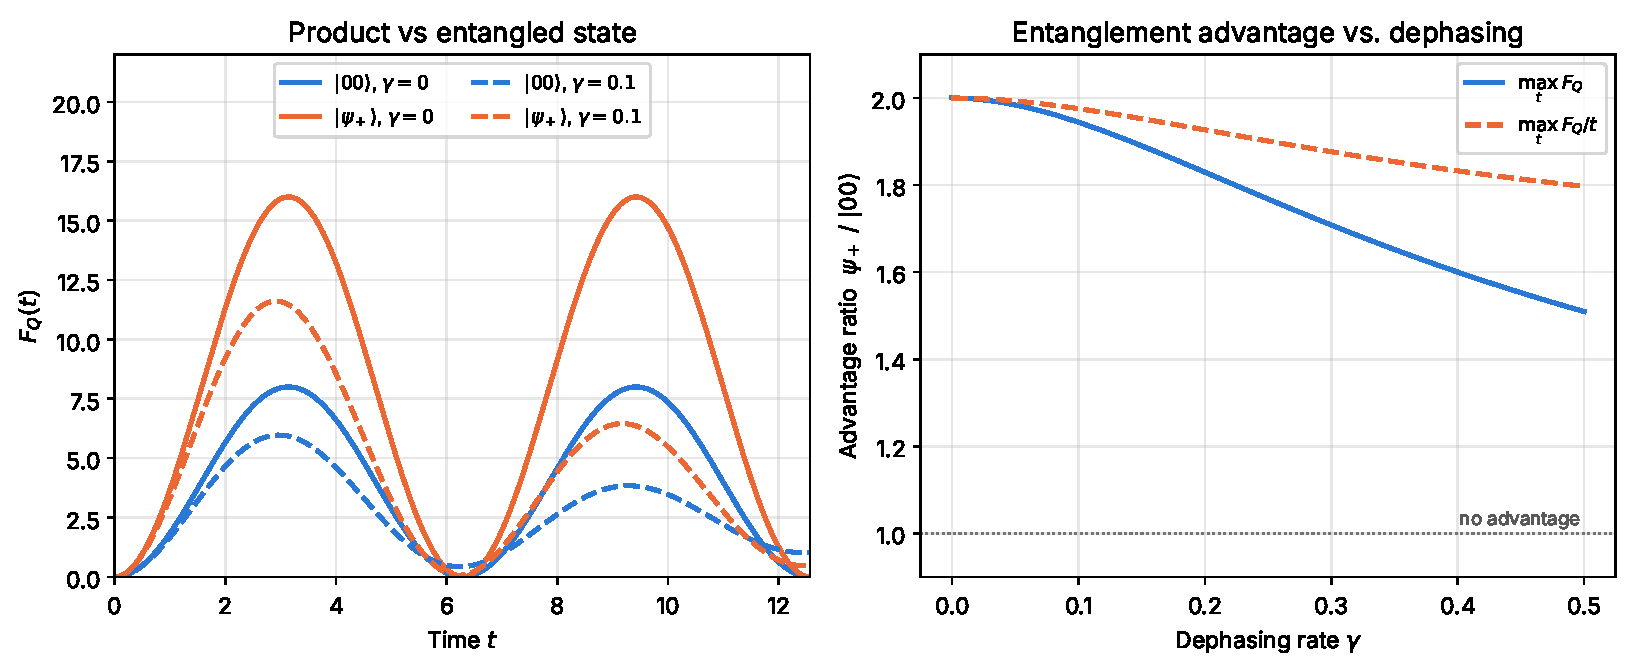
\includegraphics[width=\textwidth]{nc_comparison.pdf}
  \caption{Left: QFI of $\ket{00}$ and of $\ket{\psi_+}$ without noise (solid) and with dephasing $\gamma=0.1$ (dashed). Right: ratio between the best QFI of $\ket{\psi_+}$ and of $\ket{00}$ as a function of $\gamma$, for the maximum of $\FQ$ and for the maximum of $\FQ/t$.}
  \label{fig:comp}
\end{figure}

\begin{table}[t]
  \centering
  \begin{tabular}{@{}lccc@{}}
\toprule
$\gamma$ & $\max_t F_Q$ ratio & $\max_t F_Q/t$ ratio & time fraction with $F_{\psi_+}>F_{00}$\\
\midrule
0 & 2.00 & 2.00 & 100\%\\
0.05 & 1.99 & 2.00 & 90\%\\
0.1 & 1.94 & 1.98 & 82\%\\
0.2 & 1.83 & 1.93 & 70\%\\
0.5 & 1.51 & 1.80 & 57\%\\
\bottomrule
\end{tabular}

  \caption{Entanglement advantage of $\ket{\psi_+}$ over $\ket{00}$. The last column is the fraction of $t\in(0,4\pi]$ at which $\FQ^{(\psi_+)}>\FQ^{(00)}$.}
  \label{tab:adv}
\end{table}

% ====================================================================
\section{Discussion and outlook}\label{sec:disc}
% ====================================================================

The two-qubit XXZ model is exactly solvable and its dynamics is organised by the conserved total $S_z$. Our four initial states give no entanglement for $\ket{00}$, a full oscillation $C=\lvert\sin4Jt\rvert$ for $\ket{01}$, a reduced oscillation with $C_{\max}=1/2$ for $(\ket{00}+\ket{01})/\sqrt2$, and constant maximal entanglement for $\ket{\psi_+}$; the anisotropy appears only as phases. For the metrological problem, whether entanglement helps depends on the encoding. For a conserved generator ($S_z$) it does not: the QFI is $4t^2\Var(S_z)$ and the Bell state carries none. For a non-conserved generator ($S_x$) the Bell state has exactly twice the QFI of the product states, and $\Delta$ enters through $\omega=2J(1-\Delta)$.

Under local dephasing, entanglement-enhanced sensitivity is degraded but not destroyed. The advantage of the Bell state shrinks with $\gamma$ but remains at the best interrogation time, and it vanishes at long times, when all of $\ket{00}$, $\ket{01}$ and $\ket{\psi_+}$ reach the same QFI plateau. The best strategy is therefore to interrogate the system around the first maximum of $\FQ$, at a time of order $\pi/\omega$ or shorter. This is qualitatively consistent with the known result that, under dephasing, the advantage of entangled probes is limited to a constant factor \cite{Huelga1997,Escher2011,Demkowicz2012}.

\paragraph{Limitations.}
The initial states are pure, a single noise model (local pure dephasing in the $z$ basis) is considered, and the system has two qubits, so no scaling with the number of probes can be extracted. The long-time plateau is an empirical fit that has not been derived, and the Cram\'er--Rao bound is not shown to be attainable with a specific measurement.

\paragraph{Outlook.}
Natural extensions are initial states with support on all sectors, other noise models (amplitude damping, depolarisation, correlated dephasing), a derivation of the long-time plateau, the optimal measurement saturating the bound, and larger chains ($N>2$ qubits) to test the scaling of the QFI.

% ====================================================================
\appendix
\section{Numerical methods and validation}\label{app:num}
% ====================================================================

All numerics use QuTiP \cite{QuTiP2012} (\texttt{mesolve}, tolerances $10^{-13}$ and $10^{-11}$). Concurrence uses Wootters' formula and negativity the eigenvalues of the partial transpose. The analytic $C(t)$, $\Neg(t)$ and purities of Sec.~\ref{sec:ent} agree with the numerical ones to $4\times10^{-8}$, and the analytic $\FQ$ of Eq.~\eqref{eq:FQ} agrees with a finite-difference derivative of the evolved state to $4\times10^{-6}$.

For Sec.~\ref{sec:noncomm}, the mixed-state QFI is computed from the eigendecomposition of $\rho$ with a central finite difference of step $10^{-4}$ in $\lambda$. The checks below are run by the validation script of the repository. The QuTiP evolution agrees with an independent NumPy/SciPy implementation (exponentiation of the $16\times16$ Liouvillian) to $4\times10^{-10}$. At $\gamma=0$ the QFI agrees with the Duhamel formula to $4\times10^{-6}$ (the accuracy of the finite difference), and the Duhamel formula agrees with the closed forms~\eqref{eq:FQclosed} to $10^{-14}$. For $\gamma>0$ the QFI agrees with a superoperator pseudo-inverse implementation to $10^{-15}$ and with a fidelity-based estimate to $2.4\times10^{-3}$. The closed-form concurrences agree with Wootters' formula to $7\times10^{-10}$, and the empirical plateau holds to $10^{-5}$ for $\Delta=0,\,0.25,\,0.5,\,0.75$ and $\gamma=0.1,\,0.5$. The tables are generated by the same script that produces the figures. Code and data are in the accompanying repository.

% ====================================================================
\begin{thebibliography}{99}

\bibitem{Wootters1998} W.~K. Wootters, ``Entanglement of formation of an arbitrary state of two qubits,'' Phys.\ Rev.\ Lett.\ \textbf{80}, 2245 (1998).

\bibitem{VidalWerner2002} G.~Vidal and R.~F. Werner, ``Computable measure of entanglement,'' Phys.\ Rev.\ A \textbf{65}, 032314 (2002).

\bibitem{Horodecki2009} R.~Horodecki, P.~Horodecki, M.~Horodecki and K.~Horodecki, ``Quantum entanglement,'' Rev.\ Mod.\ Phys.\ \textbf{81}, 865 (2009).

\bibitem{BraunsteinCaves1994} S.~L. Braunstein and C.~M. Caves, ``Statistical distance and the geometry of quantum states,'' Phys.\ Rev.\ Lett.\ \textbf{72}, 3439 (1994).

\bibitem{Giovannetti2011} V.~Giovannetti, S.~Lloyd and L.~Maccone, ``Advances in quantum metrology,'' Nature Photon.\ \textbf{5}, 222 (2011).

\bibitem{Lindblad1976} G.~Lindblad, ``On the generators of quantum dynamical semigroups,'' Commun.\ Math.\ Phys.\ \textbf{48}, 119 (1976).

\bibitem{GKS1976} V.~Gorini, A.~Kossakowski and E.~C.~G. Sudarshan, ``Completely positive dynamical semigroups of $N$-level systems,'' J.\ Math.\ Phys.\ \textbf{17}, 821 (1976).

\bibitem{BreuerPetruccione2002} H.-P. Breuer and F.~Petruccione, \emph{The Theory of Open Quantum Systems} (Oxford University Press, 2002).

\bibitem{YuEberly2004} T.~Yu and J.~H. Eberly, ``Finite-time disentanglement via spontaneous emission,'' Phys.\ Rev.\ Lett.\ \textbf{93}, 140404 (2004).

\bibitem{Huelga1997} S.~F. Huelga, C.~Macchiavello, T.~Pellizzari, A.~K. Ekert, M.~B. Plenio and J.~I. Cirac, ``Improvement of frequency standards with quantum entanglement,'' Phys.\ Rev.\ Lett.\ \textbf{79}, 3865 (1997).

\bibitem{Escher2011} B.~M. Escher, R.~L. de~Matos~Filho and L.~Davidovich, ``General framework for estimating the ultimate precision limit in noisy quantum-enhanced metrology,'' Nature Phys.\ \textbf{7}, 406 (2011).

\bibitem{Demkowicz2012} R.~Demkowicz-Dobrza\'nski, J.~Ko\l ody\'nski and M.~Gu\c{t}\u{a}, ``The elusive Heisenberg limit in quantum-enhanced metrology,'' Nat.\ Commun.\ \textbf{3}, 1063 (2012).

\bibitem{QuTiP2012} J.~R. Johansson, P.~D. Nation and F.~Nori, ``QuTiP: An open-source Python framework for the dynamics of open quantum systems,'' Comput.\ Phys.\ Commun.\ \textbf{183}, 1760 (2012).

\end{thebibliography}

\end{document}
